\documentclass[a4paper, 12pt]{report}
\setlength{\parskip}{0.5em}

\usepackage{graphicx}
\usepackage[vietnamese]{babel}
\usepackage[utf8]{inputenc}
\usepackage{amsmath, amssymb}
\usepackage[top=2cm, bottom=2cm, left=2.5cm, right=2.5cm]{geometry}
\usepackage{titlesec}
\usepackage[many]{tcolorbox}
\usepackage{enumitem}
\usepackage{subcaption}
\usepackage{float}
\usepackage[hidelinks]{hyperref}
\usepackage{pgfplots}
\usepackage{tocloft}
\usepackage{minted}
\usepackage{tabularx}
\usepackage[table,xcdraw]{xcolor}
\usepackage{listings}


\hypersetup{
    colorlinks,
    linkcolor={black!50!black},
    citecolor={blue!50!black},
    urlcolor={blue!80!black}
}


\title{Báo cáo Bài tập lớn}
\author{Lâm Đức Anh}
\date{December 2024}

\newcommand{\chapnumfont}{%     % define font for chapter number
  \usefont{T1}{pnc}{b}{n}%      % choose New Chancery, bold, normal shape
  \fontsize{75}{75}%          % font size 100pt, baselineskip 100pt
  \selectfont%                  % activate font
}
\colorlet{chapnumcol}{gray!100}  % color for chapter number

\titleformat{\chapter}[display]
{\filleft\bfseries}
{\filleft\chapnumfont\textcolor{chapnumcol}{\thechapter}}
{-24pt}
{\Huge}

\setlength{\cftchapnumwidth}{3em}
\setlength{\cftbeforechapskip}{3em} 
\setlength{\cftbeforesecskip}{1em}
\setlength{\cftbeforesubsecskip}{0.5em}



\renewcommand{\thechapter}{\Roman{chapter}}
\renewcommand{\thesection}{\arabic{section}.}
\renewcommand{\thesubsection}{\alph{subsection}.}



\begin{document}


\begin{titlepage}

    \begin{center}

        % Phần trên cùng
        \textbf{\large Đại học Quốc gia Hà Nội}\\[0.2cm]
        \textbf{\large Trường Đại học Công nghệ}\\[1cm]

        
\includegraphics[width=0.2\textwidth]{UET.png}\\[2.5cm]

        % Phần ở giữa
        \textbf{\Huge BÁO CÁO BÀI TẬP LỚN}\\[0.5cm]
        \textbf{\Large Bài tập lớn Cơ sở dữ liệu}\\[2.5cm]
        
        
    \end{center}
    \vfill
    \begin{center}
        \textbf{\large Hà Nội, 2024}
    \end{center}
    
\end{titlepage}

\tableofcontents % Tạo mục lục

\newpage % Sang trang mới sau mục lục


\chapter{Đề tài}

\section{Lý do chọn đề tài}

\setlength{\parindent}{2em}

Trong thời đại công nghệ số hiện nay, các ngân hàng đang ngày càng phụ thuộc vào việc ứng dụng công nghệ thông tin để nâng cao hiệu quả hoạt động và chất lượng dịch vụ. 
Một trong những yếu tố cốt lõi để hỗ trợ các hoạt động này chính là hệ thống cơ sở dữ liệu. 
Tuy nhiên, sự phức tạp của các nghiệp vụ ngân hàng như quản lý thông tin khách hàng hay xử lý giao dịch tài chính đòi hỏi các giải pháp cơ sở dữ liệu không chỉ đảm bảo hiệu suất mà còn phải đáp ứng các yêu cầu nghiêm ngặt về tính chính xác và an toàn.

Vì vậy, nhóm đã lựa chọn đề tài \textbf{Xây dựng cơ sở dữ liệu cho Hệ thống quản lý ngân hàng}. 
Việc chọn đề tài này xuất phát từ nhu cầu thực tiễn trong ngành, khi mà các ngân hàng cần một nền tảng dữ liệu mạnh mẽ để quản lý khối lượng thông tin ngày càng lớn, hỗ trợ ra quyết định kịp thời và tối ưu hóa trải nghiệm người dùng. 

\begin{figure}[H]
    \centering
    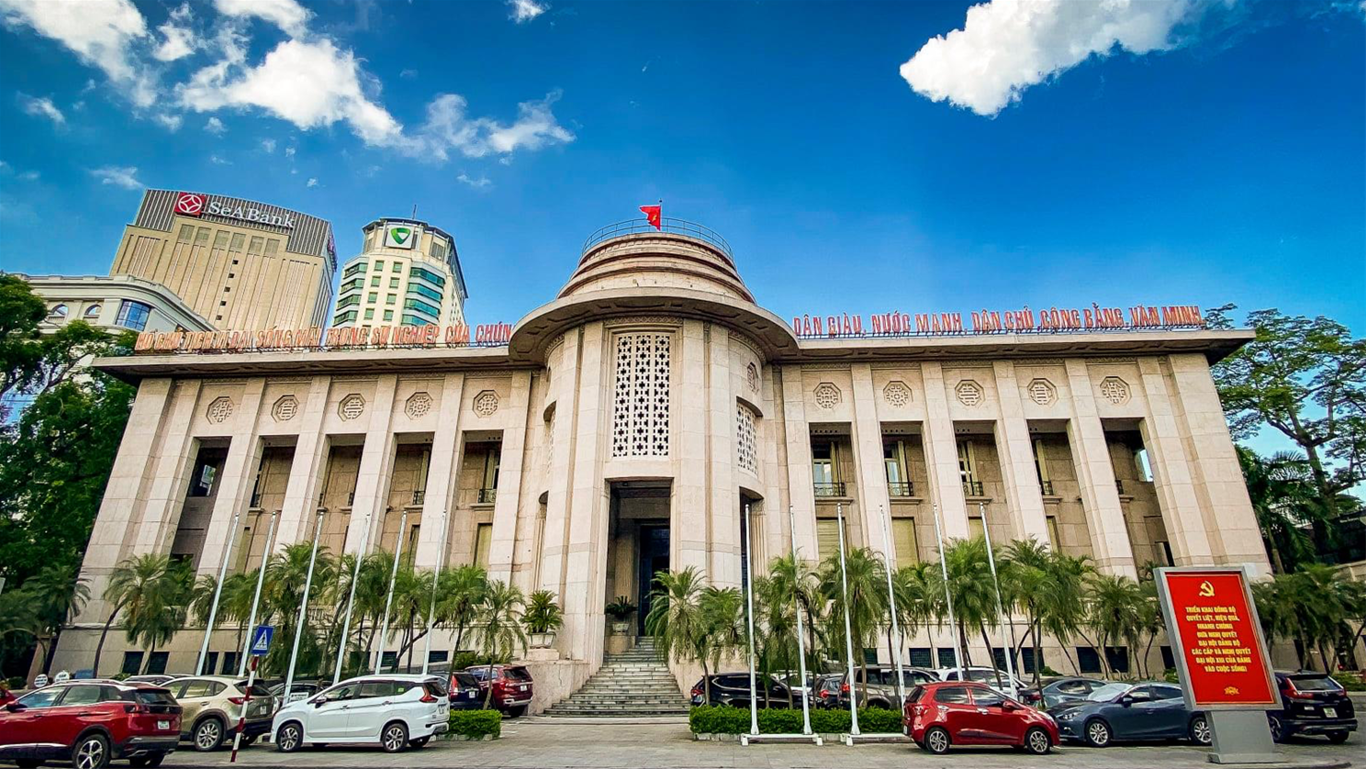
\includegraphics[width=0.8\textwidth]{CentralBank.png}
\end{figure}


\section{Phát biểu bài toán}

\textbf{Cơ sở dữ liệu dành cho hệ thống quản lý ngân hàng} được xây dựng nên để thực hiện các nhiệm vụ như lưu trữ thông tin khách hàng, quản lý 
tài khoản, xử lý các giao dịch, theo dõi các khoản vay và rủi ro tài chính, quản lý hiệu suất làm việc của nhân viên và mỗi chi nhánh trong hệ thống ngân hàng.


% \newpage
\section{Mô tả nghiệp vụ hệ thống}

Nhìn chung, một hệ thống quản lý ngân hàng sẽ bao gồm các nghiệp vụ sau đây:

\begin{enumerate}[leftmargin=2cm]

    \item \textbf{Quản lý khách hàng}: Lưu trữ thông tin cá nhân của mỗi khách hàng tại ngân hàng.
    Mỗi khách hàng là một cá nhân duy nhất và họ có thể mở nhiều tài khoản khác nhau.
    Mỗi người họ cũng có thể có những đặc điểm tài chính khác nhau và những thông tin này cần được lưu trữ để quản trị rủi ro tài chính cho ngân hàng.
    
    \item \textbf{Quản lý tài khoản}: Lưu trữ thông tin các tài khoản tại ngân hàng.
    Mỗi tài khoản là một tài sản của khách hàng nào đó gửi tại ngân hàng, chỉ được gắn với một khách hàng duy nhất.
    Tài khoản ngân hàng cũng chính là phương tiện để một khách thanh toán, nên đi kèm với tài khoản ngân hàng sẽ có những thông tin như số dư, loại hình và lịch sử giao dịch.
    
    \item \textbf{Quản lý giao dịch}: Giao dịch là nhật ký ghi lại những biến động về số dư và hướng đi của nguồn tiền trong ngân hàng.
    Mọi hoạt động tài chính của mỗi khách hàng cần phải được ghi nhận, xử lý, lưu trữ một cách chính xác và minh bạch.
    Hệ thống phải có khả năng ghi nhận các loại giao dịch khác nhau như chuyển khoản, nộp tiền, rút tiền, v.v.
    Mỗi giao dịch gắn với các thông tin như mã giao dịch, thời gian thực hiện, số tài khoản nguồn và đích, số tiền giao dịch và trạng thái giao dịch.
    
    \item \textbf{Quản lý sản phẩm tài chính}: Khi cung cấp đa dạng các dịch vụ và tiếp cận đến nhiều đối tượng khách hàng thì đòi hỏi phải có sự lưu trữ thông tin các sản phẩm này.
    Khi khách hàng mở tài khoản, thì tài khoản đó sẽ ứng với một sản phẩm tài chính nhất định.
    Ngân hàng có thể cung cấp nhiều loại sản phẩm tài chính khác nhau như tài khoản tiết kiệm, gói vay, thẻ tín dụng, v.v.
    Mỗi sản phẩm sẽ có những đặc điểm khác nhau về lãi suất, kỳ hạn và điều kiện tài chính.
    
    \item \textbf{Quản lý nhân viên và chi nhánh}: Ngân hàng được vận hành và quản lý bởi các nhân viên làm việc tại ngân hàng.
    Mỗi nhân viên phụ trách những công việc khác nhau, chủ yếu là thực hiện xử lý các giao dịch.
    Ngoài ra, ngân hàng cũng có các chi nhánh khác nhau, là nơi để các nhân viên làm việc và để khách hàng mở tài khoản.
    Việc quản lý nhân viên và chi nhánh bao gồm theo dõi công việc, đánh giá hiệu suất của mỗi nhân viên và chi nhánh.

    
\end{enumerate}


\chapter{Mô hình của hệ thống}

\section{Mô hình ER}

\begin{figure}[H]
    \centering
    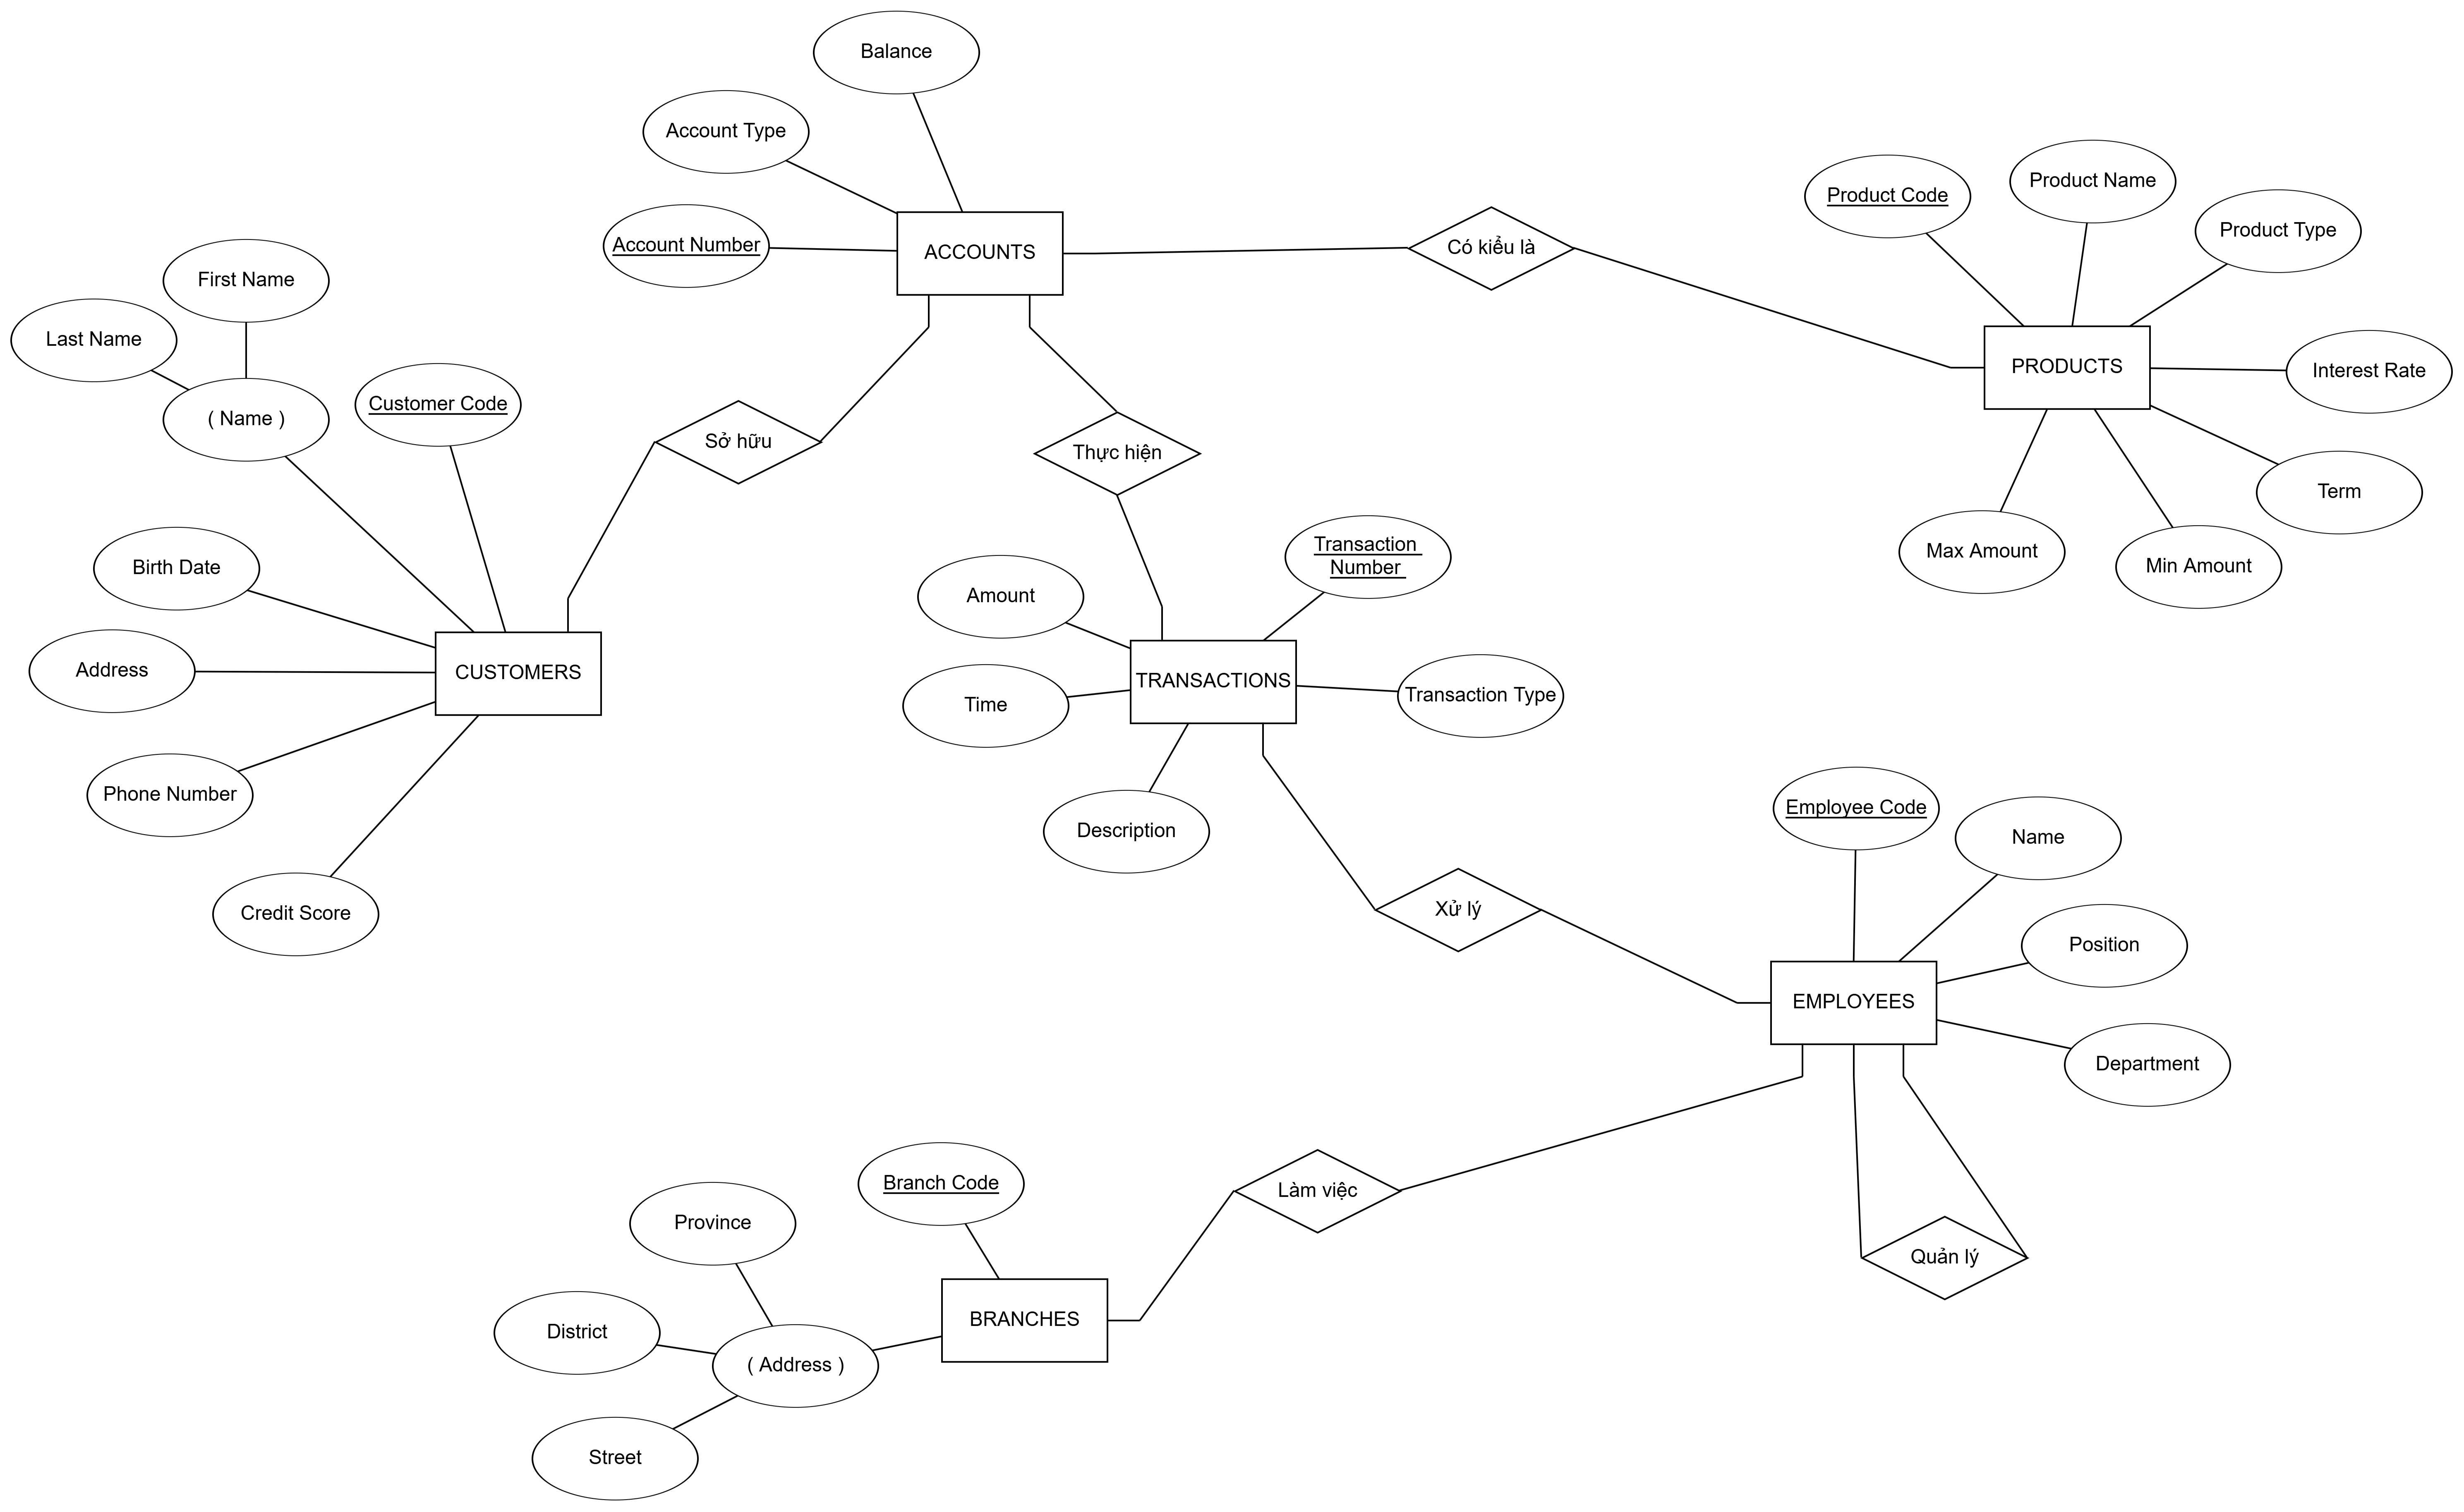
\includegraphics[width=1\textwidth]{ER-Diagram.png}
    \caption{Sơ đồ mô hình thực thể - quan hệ}
    \label{fig:br-wm-2020}
\end{figure}

\section{Mô hình quan hệ}


\chapter{Đặc tả dữ liệu}

\section{Dữ liệu tại mỗi bảng}



% \subsection{Dữ liệu Khách hàng}

Dữ liệu khách hàng được lưu trữ tại bảng \textbf{customers} với các trường dữ liệu sau:

\renewcommand{\arraystretch}{2} % Tăng khoảng cách dọc giữa các hàng
\setlength{\tabcolsep}{10pt}

\begin{center}
    \begin{tabular}{ | m{9em} | m{15em}| m{5em} | m{5em} | } 
    \hline
    \rowcolor{gray!30}
    Dữ liệu & Ý nghĩa & Kiểu & Minh họa \\ 

    \hline
    \textbf{customerID} &
    Mã định danh cho mỗi khách hàng tại ngân hàng, gồm 8 kí tự. &
    varchar &
    23020346 \\

    \hline
    \textbf{lastName} &
    Họ của khách hàng &
    varchar &
    Trần \\

    \hline
    \textbf{firstName} &
    Tên của khách hàng &
    varchar &
    Minh Huy \\

    \hline
    \textbf{birthDate} &
    Ngày tháng năm sinh của khách hàng &
    date &
    09/03/2005\\

    \hline
    \textbf{phoneNumber} &
    Số điện thoại của khách hàng &
    varchar &
    0987654321 \\

    \hline
    \textbf{address} &
    Địa chỉ của khách hàng &
    varchar &
    Cầu Giấy, Hà Nội \\

    \hline
    \textbf{creditScore} &
    Điểm tín dụng của khách hàng &
    int &
    500 \\

    \hline
    \end{tabular}
\end{center}

% \subsection{Dữ liệu tài khoản}
\newpage
\noindent
Dữ liệu tài khoản được lưu trữ tại bảng \textbf{accounts} với các trường dữ liệu sau:

\renewcommand{\arraystretch}{2} % Tăng khoảng cách dọc giữa các hàng
\setlength{\tabcolsep}{10pt}

\begin{center}
    \begin{tabular}{ | m{9em} | m{15em}| m{5em} | m{5em} | } 
    \hline
    \rowcolor{gray!30}
    Dữ liệu & Ý nghĩa & Kiểu & Minh họa \\ 

    \hline
    \textbf{accountNumber} &
    Số tài khoản, gồm 8 kí tự. &
    varchar &
    17560918 \\

    \hline
    \textbf{accountName} &
    Họ và tên của người sở hữu tài khoản &
    varchar &
    BUI THANH DAN \\

    \hline
    \textbf{balance} &
    Số dư tài khoản &
    bigint &
    5000000 \\

    \hline
    \textbf{customerID} &
    Mã định danh của khách hàng sở hữu tài khoản &
    varchar &
    23020346\\

    \hline
    \textbf{productCode} &
    Mã số sản phẩm của tài khoản &
    varchar &
    SA-103 \\

    \hline
    \textbf{openingBranch} &
    Mã chi nhánh đã mở tài khoản &
    varchar &
    QN001 \\

    \hline
    \textbf{openingDate} &
    Thời gian mở tài khoản &
    datetime &
    2017-10-15 15:28:56 \\

    \hline
    \end{tabular}
\end{center}

% \subsection{Dữ liệu chi nhánh}
\noindent
Dữ liệu chi nhánh ngân hàng được lưu trữ tại bảng \textbf{branches} với các trường dữ liệu sau:

\renewcommand{\arraystretch}{2} % Tăng khoảng cách dọc giữa các hàng
\setlength{\tabcolsep}{10pt}

\begin{center}
    \begin{tabular}{ | m{9em} | m{15em}| m{5em} | m{5em} | } 
    \hline
    \rowcolor{gray!30}
    Dữ liệu & Ý nghĩa & Kiểu & Minh họa \\ 

    \hline
    \textbf{branchCode} &
    Mã chi nhánh, gồm 5 kí tự &
    varchar &
    HN001 \\

    \hline
    \textbf{branchName} &
    Tên chi nhánh &
    varchar &
    Chi nhánh Cầu Giấy \\

    \hline
    \textbf{province} &
    Tỉnh chi nhánh hoạt động &
    varchar &
    Hà Nội \\

    \hline
    \textbf{district} &
    Huyện chi nhánh hoạt động &
    varchar &
    Cầu Giấy \\

    \hline
    \textbf{street} &
    Địa chỉ đường nơi chi nhánh tọa lạc &
    varchar &
    Số 144, đường Xuân Thủy \\

    \hline
    \end{tabular}
\end{center}




% \subsection{Dữ liệu nhân viên}
\newpage
\noindent
Dữ liệu nhân viên ngân hàng được lưu trữ tại bảng \textbf{employees} với các trường dữ liệu sau:

\renewcommand{\arraystretch}{2} % Tăng khoảng cách dọc giữa các hàng
\setlength{\tabcolsep}{10pt}

\begin{center}
    \begin{tabular}{ | m{9em} | m{15em}| m{5em} | m{5em} | } 
    \hline
    \rowcolor{gray!30}
    Dữ liệu & Ý nghĩa & Kiểu & Minh họa \\ 

    \hline
    \textbf{employeeCode} &
    Mã nhân viên, gồm 8 kí tự &
    varchar &
    14A-0007 \\

    \hline
    \textbf{lastName} &
    Họ của nhân viên &
    varchar &
    Trần \\

    \hline
    \textbf{firstName} &
    Tên của nhân viên &
    varchar &
    Ngọc Ánh \\

    \hline
    \textbf{position} &
    Chức vụ của nhân viên &
    varchar &
    Thư ký giám đốc \\

    \hline
    \textbf{department} &
    Bộ phận nhân viên làm việc &
    varchar &
    Ban giám đốc \\

    \hline
    \textbf{managerCode} &
    Mã nhân viên quản lý nhân viên này &
    varchar &
    14A-0006 \\

    \hline
    \textbf{branchCode} &
    Mã chi nhánh nhân viên làm việc &
    varchar &
    QN001 \\
    
    \hline
    \end{tabular}
\end{center}

% \subsection{Dữ liệu giao dịch}
\noindent
Dữ liệu giao dịch được lưu trữ tại bảng \textbf{transactions} với các trường dữ liệu sau:

\renewcommand{\arraystretch}{2} % Tăng khoảng cách dọc giữa các hàng
\setlength{\tabcolsep}{10pt}

\begin{center}
    \begin{tabular}{ | m{9em} | m{15em}| m{5em} | m{5em} | } 
    \hline
    \rowcolor{gray!30}
    Dữ liệu & Ý nghĩa & Kiểu & Minh họa \\ 

    \hline
    \textbf{transactionNumber} &
    Số thứ tự khi thực hiện giao dịch &
    int &
    27 \\

    \hline
    \textbf{sourceAccount} &
    Mã tài khoản chuyển tiền &
    varchar &
    70001011 \\

    \hline
    \textbf{targetAccount} &
    Mã tài khoản nhận tiền &
    varchar &
    69782850 \\

    \hline
    \textbf{transactionType} &
    Loại giao dịch &
    varchar &
    TRANSFER \\

    \hline
    \textbf{amount} &
    Số tiền giao dịch &
    bigint &
    15000000 \\

    \hline
    \textbf{time} &
    Thời gian thực hiện giao dịch thành công &
    datetime &
    2011-07-15 06:01:00 \\

    \hline
    \textbf{description} &
    Mô tả giao dịch &
    varchar &
    Vien Tri Tue Nhan Tao tra luong thang 6 \\

    \hline
    \textbf{employeeCode} &
    Mã nhân viên đã thực hiện giao dịch &
    varchar &
    30A-0003 \\

    
    \hline
    \end{tabular}
\end{center}

% \subsection{Dữ liệu dịch vụ tài khoản }
\noindent
Dữ liệu sản phẩm tài chính được lưu trữ tại bảng \textbf{products} với các trường dữ liệu sau:

\renewcommand{\arraystretch}{2} % Tăng khoảng cách dọc giữa các hàng
\setlength{\tabcolsep}{10pt}

\begin{center}
    \begin{tabular}{ | m{9em} | m{15em}| m{5em} | m{5em} | } 
    \hline
    \rowcolor{gray!30}
    Dữ liệu & Ý nghĩa & Kiểu & Minh họa \\ 

    \hline
    \textbf{productCode} &
    Mã định danh của sản phẩm &
    varchar &
    SA-102 \\

    \hline
    \textbf{productType} &
    Kiểu sản phẩm &
    varchar &
    Saving \\

    \hline
    \textbf{interestRate} &
    Lãi suất của sản phẩm, đơn vị phần trăm &
    float &
    2 \\

    \hline
    \textbf{term} &
    Kì hạn của sản phẩm  &
    int &
    3 \\

    \hline
    \textbf{minAmount} &
    Số dư tối thiểu để duy trì tài khoản với mức sản phẩm này &
    bigint &
    1000000 \\

    \hline
    \textbf{maxAmount} &
    Số tiền tối đa để tài khoản có thể duy trì sản phẩm này &
    bigint &
    100000000 \\
    
    \hline
    \end{tabular}
\end{center}

\section{Mối quan hệ giữa các bảng}

Cơ sở dữ liệu có các mối quan hệ sau:

\begin{itemize}[leftmargin=2cm]
    \item Giữa bảng \textbf{customers} và \textbf{accounts} có mối quan hệ được liên kết bởi trường
\end{itemize}

\chapter{Cài đặt}

\section{Tạo cơ sở dữ liệu và chèn dữ liệu}

\lstset{
  language=SQL,                      % Chọn ngôn ngữ SQL
  basicstyle=\ttfamily\footnotesize, % Font không chân và nhỏ gọn
  keywordstyle=\color{blue},         % Màu xanh cho từ khóa
  stringstyle=\color{red},           % Màu đỏ cho chuỗi ký tự
  frame=single,                      % Viền đơn quanh đoạn mã
  extendedchars=true,                % Hỗ trợ ký tự đặc biệt
}

\begin{enumerate}[label=\alph*.]

    \item Tạo cơ sở dữ liệu:
    
    \begin{lstlisting}
    CREATE DATABASE IF NOT EXISTS bank_db;
    \end{lstlisting}
    
    \noindent{\textbullet\ Bảng branches:}
        
    \begin{lstlisting}
    CREATE TABLE IF NOT EXISTS bank_db.branches (
        branchCode VARCHAR(50)  NOT NULL 
            PRIMARY KEY,
        branchName VARCHAR(256) NOT NULL,
        province   VARCHAR(50)  NULL,
        district   VARCHAR(50)  NULL,
        street     VARCHAR(256) NULL
    );
    \end{lstlisting}

    \noindent{\textbullet\ Bảng customers:}
        
    \begin{lstlisting}
    CREATE TABLE IF NOT EXISTS bank_db.customers (
        customerID  VARCHAR(50)  NOT NULL 
            PRIMARY KEY,
        lastName    VARCHAR(50)  NOT NULL,
        firstName   VARCHAR(50)  NOT NULL,
        birthDate   DATE         NOT NULL,
        phoneNumber VARCHAR(15)  NULL,
        address     VARCHAR(256) NULL,
        creditScore INT          NULL
    );
    \end{lstlisting}

    \newpage

    \noindent{\textbullet\ Bảng employees:}
        
    \begin{lstlisting}
    CREATE TABLE IF NOT EXISTS bank_db.employees (
        employeeCode VARCHAR(50)  NOT NULL 
            PRIMARY KEY,
        lastName     VARCHAR(50)  NOT NULL,
        firstName    VARCHAR(50)  NOT NULL,
        position     VARCHAR(256) NULL,
        department   VARCHAR(256) NULL,
        managerCode  VARCHAR(50)  NULL,
        branchCode   VARCHAR(50)  NULL
    );
    \end{lstlisting}

    \noindent{\textbullet\ Bảng products:}
        
    \begin{lstlisting}
    CREATE TABLE IF NOT EXISTS bank_db.products (
        productCode  VARCHAR(50)  NOT NULL 
            PRIMARY KEY,
        productType  VARCHAR(256) NULL,
        interestRate FLOAT        NULL,
        term         INT          NULL,
        minAmount    BIGINT       NULL,
        maxAmount    BIGINT       NULL
    );
    \end{lstlisting}

    \noindent{\textbullet\ Bảng accounts:}
        
    \begin{lstlisting}
    CREATE TABLE IF NOT EXISTS bank_db.accounts (
        accountNumber VARCHAR(256) NOT NULL 
            PRIMARY KEY,
        accountName   VARCHAR(256) NOT NULL,
        balance       BIGINT       NOT NULL,
        customerID    VARCHAR(50)  NULL,
        productCode   VARCHAR(256) NULL,
        openingBranch VARCHAR(50)  NULL,
        openingDate   DATETIME DEFAULT (NOW()) NULL
    );
    \end{lstlisting}

    \noindent{\textbullet\ Bảng transactions:}
        
    \begin{lstlisting}
    CREATE TABLE IF NOT EXISTS bank_db.transactions (
        transactionNumber INT AUTO_INCREMENT
            PRIMARY KEY,
        sourceAccount     VARCHAR(50)  NULL,
        targetAccount     VARCHAR(50)  NULL,
        transactionType   VARCHAR(50)  NULL,
        amount            BIGINT       NOT NULL,
        time              DATETIME DEFAULT 
            CURRENT_TIMESTAMP NOT NULL,
        description       VARCHAR(256) NULL,
        employeeCode      VARCHAR(50)  NULL
    );
    \end{lstlisting}
        
    \newpage

    \noindent{\textbullet\ Tạo các ràng buộc dữ liệu:}

    \begin{lstlisting}
    ALTER TABLE bank_db.employees
        ADD CONSTRAINT branch___fk
            FOREIGN KEY (branchCode) 
            REFERENCES bank_db.branches (branchCode),
        ADD CONSTRAINT employees_managers__fk
            FOREIGN KEY (managerCode) 
            REFERENCES bank_db.employees (employeeCode);

    ALTER TABLE bank_db.accounts
        ADD CONSTRAINT customerID___fk
            FOREIGN KEY (customerID) 
            REFERENCES bank_db.customers (customerID),
        ADD CONSTRAINT openingBranch___fk
            FOREIGN KEY (openingBranch) 
            REFERENCES bank_db.branches (branchCode),
        ADD CONSTRAINT productCode___fk
            FOREIGN KEY (productCode) 
            REFERENCES bank_db.products (productCode);

    ALTER TABLE bank_db.transactions
        ADD CONSTRAINT sourceAccount___fk
            FOREIGN KEY (sourceAccount) 
            REFERENCES bank_db.accounts (accountNumber),
        ADD CONSTRAINT targetAccount___fk
            FOREIGN KEY (targetAccount) 
            REFERENCES bank_db.accounts (accountNumber),
        ADD CONSTRAINT transactions__fk
            FOREIGN KEY (employeeCode) 
            REFERENCES bank_db.employees (employeeCode);
    \end{lstlisting}

    \item Chèn dữ liệu

    % \begin{figure}[H]
    %     %\centering
    %     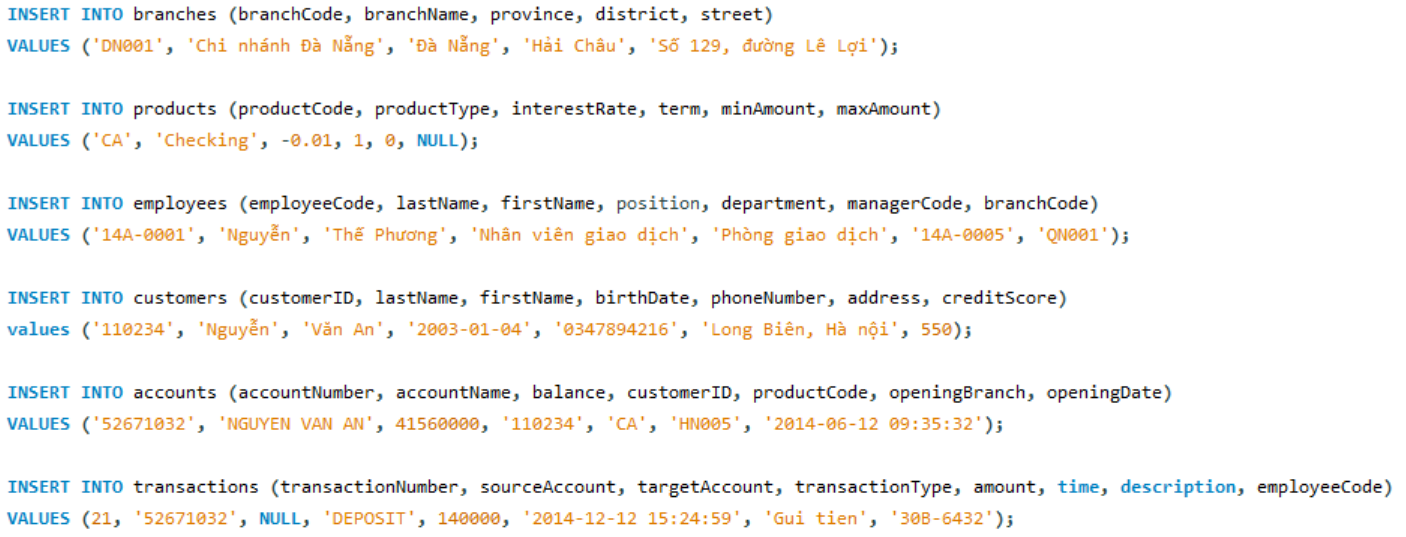
\includegraphics[width=\textwidth]{sample-insert.png}
    %     \caption{Một số ví dụ chèn dữ liệu vào các bảng.}
    %     \label{fig:sql-insert}
    % \end{figure}

    \begin{lstlisting}
    INSERT INTO branches
    (branchCode, branchName, province, district, street)
    VALUES
    ('DN001', 'Chi nhánh Đà Nẵng', 'Đà Nẵng', 'Hải Châu', 'Số 129, đường Lê Lợi');

    INSERT INTO products
    (productCode, productType, interestRate, term, minAmount, maxAmount)
    VALUES 
    ('CA', 'Checking', -0.01, 1, 0, NULL);

    INSERT INTO employees
    (employeeCode, lastName, firstName, position, department, managerCode, branchCode)
    VALUES 
    ('14A-0001', 'Nguyễn', 'Thế Phương', 'Nhân viên giao dịch', 'Phòng giao dịch', '14A-0005', 'QN001');

    INSERT INTO customers
    (customerID, lastName, firstName, birthDate, phoneNumber, address, creditScore)
    VALUES
    ('110234', 'Nguyễn', 'Văn An', '2003-01-04', '0347894216', 'Long Biên, Hà nội', 550);

    INSERT INTO accounts
    (accountNumber, accountName, balance, customerID, productCode, openingBranch, openingDate)
    VALUES
    ('52671032', 'NGUYEN VAN AN', 41560000, '110234', 'CA', 'HN005', '2014-06-12 09:35:32');

    INSERT INTO transactions
    (transactionNumber, sourceAccount, targetAccount, transactionType, amount, time, description, employeeCode)
    VALUES
    (21, '52671032', NULL, 'DEPOSIT', 140000, '2014-12-12 15:24:59', 'Gui tien', '30B-6432');
    \end{lstlisting}
 
\end{enumerate}


\section{Truy vấn dữ liệu}

\newminted[MySQLCode]{sql}{
    frame=single, % Viền bao quanh mã
    framesep=2mm, % Khoảng cách giữa mã và viền
    fontsize=\scriptsize, % Kích thước chữ nhỏ hơn  footnotesize
    baselinestretch=1.1, % Dãn dòng vừa phải
    breaklines, % Tự động xuống dòng
    tabsize=3, % Kích thước tab
    autogobble % Loại bỏ khoảng trắng thừa
}

TRUY VẤN KHÁCH HÀNG:
\begin{itemize}

    \item Truy vấn xem mỗi khách hàng có bao nhiêu tài khoản (group by + inner join + aggregate functions)
    \begin{MySQLCode}
    SELECT 
        c.customerID,
        CONCAT(c.lastName, ' ', c.firstName) AS customerName,
        COUNT(a.accountNumber) AS totalAccounts
    FROM 
        bank_db.customers c
    JOIN 
        bank_db.accounts a ON c.customerID = a.customerID
    GROUP BY 
        c.customerID;
    \end{MySQLCode}

    \item Truy vấn tính tổng số tiền trong tất cả tài khoản của mỗi khách hàng (group by + inner join + aggregate functions)
    \begin{MySQLCode}
    SELECT 
        c.customerID,
	CONCAT(c.lastName, ' ', c.firstName) AS customerName,
        SUM(a.balance) AS totalBalance
    FROM 
        bank_db.customers c
    JOIN 
        bank_db.accounts a ON c.customerID = a.customerID
    GROUP BY 
	c.customerID;
    \end{MySQLCode}

    \item Truy vấn tìm khách hàng có sinh nhật vào quý 4
    \begin{MySQLCode}
    SELECT 
        customerID,
        CONCAT(lastName, ' ', firstName) AS customerName,
        birthDate
    FROM 
        bank_db.customers
    WHERE 
        MONTH(birthDate) IN (10, 11, 12);
    \end{MySQLCode}

    \item Truy vấn tìm khách hàng có sinh nhật vào quý 4
    \begin{MySQLCode}
    SELECT 
        customerID,
        CONCAT(lastName, ' ', firstName) AS customerName,
        birthDate
    FROM 
        bank_db.customers
    WHERE 
        MONTH(birthDate) IN (10, 11, 12);
    \end{MySQLCode}

     \item Truy vấn số lượng khách hàng ở mỗi thang điểm tín dụng (group by + aggregate functions)
    \begin{MySQLCode}
    SELECT 
        creditScore,
        COUNT(*) AS customerCount
    FROM 
        bank_db.customers
    GROUP BY 
        creditScore
    ORDER BY 
        creditScore;
    \end{MySQLCode}

    \item Truy vấn mỗi khách hàng đã thực hiện bao nhiêu giao dịch (inner join + group by + aggregate functions)
    \begin{MySQLCode}
    SELECT 
        c.customerID,
        CONCAT(c.lastName, ' ', c.firstName) AS customerName,
        COUNT(*) AS totalTransactions
    FROM
	bank_db.customers c
    JOIN
        bank_db.accounts a ON c.customerID = a.customerID
    JOIN 
        bank_db.transactions t ON a.accountNumber = t.sourceAccount OR a.accountNumber = t.targetAccount
    GROUP BY 
        c.customerID;
    \end{MySQLCode}

    \item Truy vẫn tất cả tài khoản và số dư trong đó của mỗi khách hàng (outer join + aggregate functions)
    \begin{MySQLCode}
    SELECT 
        c.customerID,
        CONCAT(c.lastName, ' ', c.firstName) AS customerName,
        a.accountNumber,
        a.balance
    FROM 
        bank_db.customers c
    LEFT JOIN 
        bank_db.accounts a ON c.customerID = a.customerID

    UNION

    SELECT 
        c.customerID,
        CONCAT(c.lastName, ' ', c.firstName) AS customerName,
        a.accountNumber,
        a.balance
    FROM 
        bank_db.customers c
    RIGHT JOIN 
        bank_db.accounts a ON c.customerID = a.customerID;
    \end{MySQLCode}

    \item Truy vấn mỗi khách hàng đã được phục vụ bởi bao nhiêu nhân viên (inner join + group by + aggregate functions)
    \begin{MySQLCode}
    SELECT 
        c.customerID,
        CONCAT(c.lastName, ' ', c.firstName) AS customerName,
        COUNT(DISTINCT t.employeeCode) AS totalEmployees
    FROM 
        bank_db.customers c
    JOIN 
        bank_db.accounts a ON c.customerID = a.customerID
    JOIN 
        bank_db.transactions t ON a.accountNumber = t.sourceAccount OR a.accountNumber = t.targetAccount
    GROUP BY 
        c.customerID;
    \end{MySQLCode}

\end{itemize}
TRUY VẤN TÀI KHOẢN:
\begin{itemize}

    \item Truy vấn mỗi tài khoản đã thực hiện bao nhiêu giao dịch chuyển tiền (group by + inner join + aggregate functions)
    \begin{MySQLCode}
    SELECT 
        a1.accountNumber,
        a1.accountName,
        COUNT(t1.transactionNumber) AS totalTransactions
    FROM 
        bank_db.accounts a1
    JOIN 
        bank_db.transactions t1 ON a1.accountNumber = t1.sourceAccount
    GROUP BY 
        a1.accountNumber;
    \end{MySQLCode}

    \item Truy vấn mỗi tài khoản đã thực hiện chuyển hay rút bao nhiêu tiền (group by + inner join + aggregate functions)
    \begin{MySQLCode}
    SELECT 
        a1.accountNumber,
        a1.accountName,
        SUM(t1.amount) AS totalTransactionsAmount
    FROM 
        bank_db.accounts a1
    JOIN 
        bank_db.transactions t1 ON a1.accountNumber = t1.sourceAccount
    GROUP BY 
        a1.accountNumber;
    \end{MySQLCode}

    \item Truy vấn mỗi tài khoản đã chuyển nhiều tiền nhất cho tài khoản nào khác null (subquery trong from và where + aggregate functions + group by)
    \begin{MySQLCode}
    SELECT 
        t1.sourceAccount, 
        t1.targetAccount, 
        t1.totalAmount
    FROM (
        SELECT 
            sourceAccount, 
            targetAccount, 
            SUM(amount) AS totalAmount
        FROM 
            bank_db.transactions
        WHERE 
            sourceAccount IS NOT NULL 
            AND targetAccount IS NOT NULL 
            AND amount IS NOT NULL
        GROUP BY 
            sourceAccount, targetAccount
    ) t1
    WHERE 
        t1.totalAmount = (
            SELECT 
                MAX(t2.totalAmount)
            FROM (
                SELECT 
                    sourceAccount, 
                    targetAccount, 
                    SUM(amount) AS totalAmount
                FROM 
                    bank_db.transactions
                WHERE 
                    sourceAccount IS NOT NULL 
                    AND targetAccount IS NOT NULL 
                    AND amount IS NOT NULL
                GROUP BY 
                    sourceAccount, targetAccount
            ) t2
            WHERE 
                t2.sourceAccount = t1.sourceAccount
        );
    \end{MySQLCode}

    \item Truy vẫn mỗi tài khoản đã thực hiện nhiều giao dịch chuyển tiền nhất cho tài khoản nào khác null (subquery trong from và where + aggregate functions + group by)
    \begin{MySQLCode}
    SELECT 
        t1.sourceAccount, 
        t1.targetAccount, 
        t1.transactionCount
    FROM (
        SELECT 
            sourceAccount, 
            targetAccount, 
            COUNT(*) AS transactionCount
        FROM 
            bank_db.transactions
        WHERE 
            sourceAccount IS NOT NULL 
            AND targetAccount IS NOT NULL
        GROUP BY 
            sourceAccount, targetAccount
    ) t1
    WHERE 
        t1.transactionCount = (
            SELECT 
                MAX(t2.transactionCount)
            FROM (
                SELECT 
                    sourceAccount, 
                    targetAccount, 
                    COUNT(*) AS transactionCount
                FROM 
                    bank_db.transactions
                WHERE 
                    sourceAccount IS NOT NULL 
                    AND targetAccount IS NOT NULL
                GROUP BY 
                    sourceAccount, targetAccount
            ) t2
            WHERE 
                t2.sourceAccount = t1.sourceAccount
        );
    \end{MySQLCode}

    \item Truy vấn số lượng tài khoản được mở mỗi năm (group by + aggregate functions)
    \begin{MySQLCode}
    SELECT 
        YEAR(openingDate) AS openingYear,
        COUNT(*) AS accountCount
    FROM 
        bank_db.accounts
    WHERE 
        openingDate IS NOT NULL
    GROUP BY 
        YEAR(openingDate)
    ORDER BY 
        openingYear;
    \end{MySQLCode}

\end{itemize}
TRUY VẤN NHÂN VIÊN:
\begin{itemize}

   \item Truy vấn nhân viên và tất cả người quản lý của họ (self join + aggregate functions)
    \begin{MySQLCode}
    SELECT 
        e.employeeCode,
        CONCAT(e.lastName, ' ', e.firstName) AS employeeName,
        m.employeeCode AS managerCode,
        CONCAT(m.lastName, ' ', m.firstName) AS managerName
    FROM 
        bank_db.employees e
    LEFT JOIN 
        bank_db.employees m ON e.managerCode = m.employeeCode;
    \end{MySQLCode}

    \item Truy vấn nhân viên và số cấp dưới họ quản lý (self join + group by + aggregate functions)
    \begin{MySQLCode}
    SELECT 
        e1.employeeCode AS managerCode,
        CONCAT(e1.lastName, ' ', e1.firstName) AS managerName,
        COUNT(e2.employeeCode) AS subordinateCount
    FROM 
        bank_db.employees e1
    LEFT JOIN 
        bank_db.employees e2 ON e1.employeeCode = e2.managerCode
    GROUP BY 
        e1.employeeCode
    ORDER BY 
        subordinateCount DESC;
    \end{MySQLCode}

    \item Truy vấn nhân viên và tổng số tiền giao dịch họ đã xử lý (inner join + group by + aggregate functions)
    \begin{MySQLCode}
    SELECT 
        e.employeeCode,
        CONCAT(e.lastName, ' ', e.firstName) AS employeeName,
	SUM(t.amount) AS totalRevenue
    FROM 
        bank_db.employees e
    JOIN 
        bank_db.transactions t ON t.employeeCode = e.employeeCode
    GROUP BY 
        e.employeeCode
    ORDER BY 
        totalRevenue DESC
    \end{MySQLCode}

    \item Truy vấn mỗi nhân viên đã từng phục vụ bao nhiêu khách hàng (inner join + group by + aggregate functions)
    \begin{MySQLCode}
    SELECT 
        e.employeeCode,
        CONCAT(e.lastName, ' ', e.firstName) AS employeeName,
        COUNT(*) AS totalCustomers
    FROM
	bank_db.employees e
    JOIN
        bank_db.transactions t ON e.employeeCode = t.employeeCode
    JOIN 
        bank_db.accounts a ON a.accountNumber = t.sourceAccount OR a.accountNumber = t.targetAccount
    GROUP BY 
        e.employeeCode;
    \end{MySQLCode}

\end{itemize}
TRUY VẤN GIAO DỊCH:
\begin{itemize}

    \item Truy vấn tính số lượng giao dịch trong mỗi năm (group by + aggregate functions)
    \begin{MySQLCode}
    SELECT 
        YEAR(time) AS Year,
        COUNT(*) AS transactionCount
    FROM 
        bank_db.transactions
    GROUP BY 
        YEAR
    ORDER BY 
        Year;
    \end{MySQLCode}

    \item Truy vấn số lượng tiền vào mỗi tháng (group by + aggregate functions)
    \begin{MySQLCode}
    SELECT 
        DATE_FORMAT(time, '%Y-%m') AS month, 
        SUM(amount) AS totalAmount
    FROM 
        bank_db.transactions
    WHERE 
        amount IS NOT NULL
        AND transactionType IN ('DEPOSIT')
    GROUP BY 
        month
    ORDER BY 
        totalAmount;
    \end{MySQLCode}
    
    \item Truy vấn số lượng tiền ra mỗi tháng (group by + aggregate functions)
    \begin{MySQLCode}
    SELECT 
        DATE_FORMAT(time, '%Y-%m') AS month, 
        SUM(amount) AS totalAmount
    FROM 
        bank_db.transactions
    WHERE 
        amount IS NOT NULL
        AND transactionType = 'WITHDRAW'
    GROUP BY 
        month
    ORDER BY 
        totalAmount;
    \end{MySQLCode}

    \item Truy vấn tổng số tiền của mỗi loại giao dịch (group by + aggregate functions)
    \begin{MySQLCode}
    SELECT 
        transactionType, 
        SUM(amount) AS totalAmount
    FROM 
        bank_db.transactions
    WHERE 
        amount IS NOT NULL
    GROUP BY 
        transactionType
    ORDER BY 
        totalAmount DESC;
    \end{MySQLCode}

\end{itemize}
TRUY VẤN CHI NHÁNH:
\begin{itemize}

     \item Truy vấn mỗi chi nhánh có tất cả bao nhiêu nhân viên (inner join + group by + aggregate functions)
    \begin{MySQLCode}
    SELECT 
        b1.branchCode,
        b1.branchName,
        COUNT(e1.employeeCode) AS totalEmployee
    FROM 
        bank_db.branches b1
    JOIN 
        bank_db.employees e1 ON b1.branchCode = e1.branchCode
    GROUP BY 
        b1.branchCode;
    \end{MySQLCode}

    \item Truy vấn tổng số tiền các giao dịch rút tiền, chuyển tiền, nạp tiền đã thực hiện tại mỗi chi nhánh (inner join + group by + aggregate functions)
    \begin{MySQLCode}
    SELECT 
        b.branchName AS branchName,
        t.transactionType,
        SUM(t.amount) AS totalAmount
    FROM 
        bank_db.transactions t
    JOIN 
        bank_db.employees e ON t.employeeCode = e.employeeCode
    JOIN 
        bank_db.branches b ON e.branchCode = b.branchCode
    WHERE 
        t.amount IS NOT NULL
        AND t.transactionType IN ('WITHDRAW', 'TRANSFER', 'DEPOSIT')
    GROUP BY 
        b.branchName, t.transactionType
    ORDER BY 
        b.branchName, t.transactionType;
    \end{MySQLCode}

    \item Truy vấn số tài khoản được mở tại mỗi chi nhánh (inner join + group by + aggregate functions)
    \begin{MySQLCode}
    SELECT 
	a.openingBranch, 
        b.branchName,
        COUNT(*) AS totalAccounts
    FROM 
	bank_db.accounts a
    JOIN
	bank_db.branches b ON a.openingBranch = b.branchCode
    GROUP BY
	openingBranch;
    \end{MySQLCode}

    \item Truy vấn số nhân viên trong từng chức vụ tại mỗi chi nhánh (inner join + group by + aggregate functions)
    \begin{MySQLCode}
    SELECT 
	b.branchCode,
        b.branchName,
        e.position,
        COUNT(*) AS totalEmployees
    FROM 
        bank_db.employees e
    JOIN 
        bank_db.branches b ON e.branchCode = b.branchCode
    GROUP BY 
        b.branchCode, e.position;
    \end{MySQLCode}

    \item Truy vấn các chi nhánh và tên đầy đủ của giám đốc chi nhánh đó (inner join + aggregate functions)
    \begin{MySQLCode}
    SELECT 
	b.branchCode,
        b.branchName,
        CONCAT(e.lastName, ' ', e.firstName) as directorName
    FROM 
        bank_db.employees e
    JOIN 
        bank_db.branches b ON e.branchCode = b.branchCode
    WHERE
    	e.position = 'Giám đốc chi nhánh'
    \end{MySQLCode}

    \item Truy vấn số lượng chi nhánh tại mỗi tỉnh thành (group by + aggregate functions)
    \begin{MySQLCode}
    SELECT 
	province,
        COUNT(*) AS totalBranches
    FROM 
        bank_db.branches
    GROUP BY 
        province;
    \end{MySQLCode}

\end{itemize}
TRUY VẤN SẢN PHẨM:
\begin{itemize}

    \item Truy vấn mỗi sản phẩm có bao nhiêu tài khoản (inner join + group by + aggregate functions)
    \begin{MySQLCode}
    SELECT
	p.productCode,
        p.productType,
        COUNT(*) AS totalAccounts
    FROM 
	bank_db.products p
    JOIN
	bank_db.accounts a ON a.productCode = p.productCode
    GROUP BY
	p.productCode;
    \end{MySQLCode}

    \item Truy vấn mỗi khách hàng yêu thích sản phẩm nào nhất (giả sử sản phẩm nào khách hàng có nhiều tài khoản nhất thì là yêu thích nhất)(inner join + subquery trong from + group by + aggregate functions)
    \begin{MySQLCode}
    SELECT
        c.customerID,
        CONCAT(c.lastName, ' ', c.firstName) AS customerName,
        p.productCode,
        p.productType,
        COUNT(*) AS totalAccounts
    FROM
        bank_db.customers c
    JOIN 
        bank_db.accounts a ON c.customerID = a.customerID
    JOIN 
        bank_db.products p ON a.productCode = p.productCode
    GROUP BY
        c.customerID,
        p.productCode,
        p.productType
    HAVING
        COUNT(*) = (
            SELECT 
                MAX(account_count)
            FROM (
                SELECT 
                    c2.customerID,
                    p2.productCode,
                    COUNT(*) AS account_count
                FROM
                    bank_db.customers c2
                JOIN 
                    bank_db.accounts a2 ON c2.customerID = a2.customerID
                JOIN 
                    bank_db.products p2 ON a2.productCode = p2.productCode
                GROUP BY
                    c2.customerID,
                    p2.productCode
            ) AS subquery_max
            WHERE subquery_max.customerID = c.customerID
        );
    \end{MySQLCode}

\end{itemize}

    
    

    



\section{Ràng buộc dữ liệu bằng trigger}

\newminted[MySQLCode]{sql}{
    frame=single, % Viền bao quanh mã
    framesep=2mm, % Khoảng cách giữa mã và viền
    fontsize=\scriptsize, % Kích thước chữ nhỏ hơn  footnotesize
    baselinestretch=1.1, % Dãn dòng vừa phải
    breaklines, % Tự động xuống dòng
    tabsize=3, % Kích thước tab
    autogobble % Loại bỏ khoảng trắng thừa
}

\begin{itemize}

    \item Trigger \texttt{before\_transaction\_validation} giúp kiểm tra xem các tài khoản đã tồn tại trên hệ thống hay chưa trước khi thực hiện giao dịch:
    \begin{MySQLCode}
    CREATE TRIGGER before_transaction_validation
    BEFORE INSERT ON transactions
    FOR EACH ROW
    BEGIN
        -- Kiểm tra nếu là giao dịch gửi tiền
        IF NEW.transactionType = 'DEPOSIT' THEN
            IF NOT EXISTS (
                SELECT 1 FROM accounts WHERE accountNumber = NEW.targetAccount
            ) THEN
                SIGNAL SQLSTATE '45000'
                SET MESSAGE_TEXT = 'Giao dịch thất bại: Tài khoản đích không tồn tại.';
            END IF;
        END IF;

        -- Kiểm tra nếu là giao dịch rút tiền
        IF NEW.transactionType = 'WITHDRAW' THEN
            IF NOT EXISTS (
                SELECT 1 FROM accounts WHERE accountNumber = NEW.sourceAccount
            ) THEN
                SIGNAL SQLSTATE '45000'
                SET MESSAGE_TEXT = 'Giao dịch thất bại: Tài khoản nguồn không tồn tại.';
            END IF;
        END IF;

        -- Kiểm tra nếu là giao dịch chuyển tiền
        IF NEW.transactionType = 'TRANSFER' THEN
            -- Kiểm tra tài khoản nguồn
            IF NOT EXISTS (
                SELECT 1 FROM accounts WHERE accountNumber = NEW.sourceAccount
            ) THEN
                SIGNAL SQLSTATE '45000'
                SET MESSAGE_TEXT = 'Giao dịch thất bại: Tài khoản nguồn không tồn tại.';
            END IF;

            -- Kiểm tra tài khoản đích
            IF NOT EXISTS (
                SELECT 1 FROM accounts WHERE accountNumber = NEW.targetAccount
            ) THEN
                SIGNAL SQLSTATE '45000'
                SET MESSAGE_TEXT = 'Giao dịch thất bại: Tài khoản đích không tồn tại.';
            END IF;
        END IF;
    END;
    \end{MySQLCode}

    \newpage

    \item Trigger \texttt{before\_transaction\_check} yêu cầu với số tiền giao dịch tối thiểu đối với mỗi loại giao dịch:
    \begin{MySQLCode}
    CREATE TRIGGER before_transaction_check
    BEFORE INSERT ON transactions
    FOR EACH ROW
    BEGIN
        -- Kiểm tra nếu là giao dịch rút tiền hoặc chuyển khoản
        IF NEW.transactionType IN ('WITHDRAW', 'TRANSFER') THEN
            -- Đảm bảo số tiền rút hoặc chuyển đi là ít nhất 10,000
            IF NEW.amount < 10000 THEN
                SIGNAL SQLSTATE '45000'
                SET MESSAGE_TEXT = 'Giao dịch thất bại: Số tiền trong một giao dịch chuyển tiền/rút tiền tối thiểu 10,000 VND.';
            END IF;
        END IF;

        -- Kiểm tra nếu là gửi tiền thì số tiền phải ít nhất là 50,000
        IF NEW.transactionType = 'DEPOSIT' THEN
            IF NEW.amount < 50000 THEN
                SIGNAL SQLSTATE '45000'
                SET MESSAGE_TEXT = 'Giao dịch thất bại: Số tiền trong một giao dịch gửi tiền tối thiểu 50,000 VND.';
            END IF;
        END IF;
    END;
    \end{MySQLCode}
    
    \item Trigger \texttt{before\_withdraw\_or\_transfer} thực hiện kiểm tra số dư tài khoản nguồn có đủ để thực hiện các giao dịch như rút tiền hoặc chuyển khoản:
    \begin{MySQLCode}
    CREATE TRIGGER before_withdraw_or_transfer
    BEFORE INSERT ON transactions
    FOR EACH ROW
    BEGIN
        DECLARE current_balance BIGINT;
        -- Kiểm tra nếu là giao dịch chuyển khoản
        IF NEW.transactionType IN ('WITHDRAW', 'TRANSFER') THEN
            -- Lấy số dư hiện tại của tài khoản nguồn
            SELECT balance INTO current_balance
            FROM accounts
            WHERE accountNumber = NEW.sourceAccount;

            -- Nếu số dư không đủ thì chặn giao dịch
            IF current_balance < NEW.amount THEN
                SIGNAL SQLSTATE '45000'
                SET MESSAGE_TEXT = 'Giao dịch thất bại: Số dư không đủ.';
            END IF;
        END IF;
    END;
    \end{MySQLCode}

    \item Trigger \texttt{after\_deposit} sẽ tự động cập nhật số dư tài khoản sau một giao dịch nạp tiền:
    \begin{MySQLCode}
    CREATE TRIGGER after_deposit
    AFTER INSERT ON transactions
    FOR EACH ROW
    BEGIN
        IF NEW.transactionType = 'DEPOSIT' THEN
            -- Cập nhật số dư của tài khoản khi có giao dịch nạp tiền
            UPDATE accounts
            SET balance = balance + NEW.amount
            WHERE accountNumber = NEW.targetAccount;
        END IF;
    END;
    \end{MySQLCode}

    \item Trigger \texttt{after\_withdraw} sẽ tự động cập nhật số dư tài khoản sau một giao dịch rút tiền:
    \begin{MySQLCode}
    CREATE TRIGGER after_withdraw
    AFTER INSERT ON transactions
    FOR EACH ROW
    BEGIN
        IF NEW.transactionType = 'WITHDRAW' THEN
            -- Trừ tiền từ tài khoản nguồn
            UPDATE accounts
            SET balance = balance - NEW.amount
            WHERE accountNumber = NEW.sourceAccount;
        END IF;
    END;
    \end{MySQLCode}
    
    \item Trigger \texttt{after\_transfer} sẽ tự động cập nhật số dư của 2 tài khoản sau một giao dịch chuyển khoản:
    \begin{MySQLCode}
    CREATE TRIGGER after_transfer
    AFTER INSERT ON transactions
    FOR EACH ROW
    BEGIN
        IF NEW.transactionType = 'TRANSFER' THEN
            -- Trừ tiền từ tài khoản nguồn
            UPDATE accounts
            SET balance = balance - NEW.amount
            WHERE accountNumber = NEW.sourceAccount;

            -- Cộng tiền vào tài khoản đích
            UPDATE accounts
            SET balance = balance + NEW.amount
            WHERE accountNumber = NEW.targetAccount;
        END IF;
    END;
    \end{MySQLCode}

    \item Trigger \texttt{before\_account\_creation} thực hiển kiểm tra điểm tín dụng của một khách hàng liệu có đủ điều kiện để mở tài khoản hay không:
    \begin{MySQLCode}
    CREATE TRIGGER before_account_creation
    BEFORE INSERT ON accounts
    FOR EACH ROW
    BEGIN
        DECLARE credit_score INT;
        -- Kiểm tra xem customerID có tồn tại trong bảng customers không
        IF NOT EXISTS (
            SELECT 1 FROM customers WHERE customerID = NEW.customerID
        ) THEN
            SIGNAL SQLSTATE '45000'
            SET MESSAGE_TEXT = 'Khách hàng không tồn tại trong hệ thống.';
        ELSE
            -- Lấy điểm tín dụng của khách hàng
            SELECT creditScore INTO credit_score
            FROM customers
            WHERE customerID = NEW.customerID;

            -- Kiểm tra điểm tín dụng
            IF credit_score < 300 THEN
                SIGNAL SQLSTATE '45000'
                SET MESSAGE_TEXT = 'Điểm tín dụng không đủ để mở tài khoản.';
            END IF;
        END IF;
    END;
    \end{MySQLCode}
    
\end{itemize}

\section{Giải quyết nghiệp vụ bằng procedures}

\newminted[MySQLCode]{sql}{
    frame=single, % Viền bao quanh mã
    framesep=2mm, % Khoảng cách giữa mã và viền
    fontsize=\scriptsize, % Kích thước chữ nhỏ hơn  footnotesize
    baselinestretch=1.1, % Dãn dòng vừa phải
    breaklines, % Tự động xuống dòng
    tabsize=3, % Kích thước tab
    autogobble % Loại bỏ khoảng trắng thừa
}

\begin{itemize}

    \item Procedure \texttt{GetAccountsByCustomerID} hiển thị thông tin tài khoản của một khách hàng, thông qua mã khách hàng:
    \begin{MySQLCode}
    CREATE PROCEDURE GetAccountsByCustomerID(
        IN p_customerID VARCHAR(50)
    )
    BEGIN
        SELECT accountNumber, accountName, balance, productCode, openingBranch, openingDate
        FROM accounts
        WHERE customerID = p_customerID;
    END;
    \end{MySQLCode}

    \item Procedure \texttt{GetTransactionHistory} hiển thị lịch sử giao dịch của một tài khoản, thông qua số tài khoản:
    \begin{MySQLCode}
    CREATE PROCEDURE GetTransactionHistory(
        IN p_accountNumber VARCHAR(50)
    )
    BEGIN
        SELECT transactionNumber, sourceAccount, targetAccount, transactionType, amount, time, description
        FROM transactions
        WHERE sourceAccount = p_accountNumber OR targetAccount = p_accountNumber
        ORDER BY time DESC;
    END;
    \end{MySQLCode}

    \item Procedure \texttt{GetEmployeesByBranch} lấy danh sách nhân viên của một chi nhánh, thông qua mã chi nhánh:
    \begin{MySQLCode}
    CREATE PROCEDURE GetEmployeesByBranch(
        IN p_branchCode VARCHAR(50)
    )
    BEGIN
        SELECT employeeCode, CONCAT(lastName, ' ', firstName) as FullName, position, department, managerCode
        FROM employees
        WHERE branchCode = p_branchCode;
    END;
    \end{MySQLCode}

    \item Procedure \texttt{GetTransactionsBySpecificDate} đưa ra danh sách các giao dịch trong một ngày, tháng hoặc năm cụ thể:
    \begin{MySQLCode}
    CREATE PROCEDURE GetTransactionsBySpecificDate(
        IN p_year INT,      -- Có thể NULL
        IN p_month INT,     -- Có thể NULL
        IN p_day INT        -- Có thể NULL
    )
    BEGIN
        SELECT transactionNumber, sourceAccount, targetAccount, transactionType, amount, time, description, employeeCode
        FROM transactions
        WHERE
            (p_year IS NULL OR YEAR(time) = p_year) AND
            (p_month IS NULL OR MONTH(time) = p_month) AND
            (p_day IS NULL OR DAY(time) = p_day)
        ORDER BY time;
    END;
    \end{MySQLCode}

    \item Procedure \texttt{AddNewCustomer} thực hiện thêm một khách hàng mới vào hệ thống:
    \begin{MySQLCode}
    CREATE PROCEDURE AddNewCustomer(
        IN p_customerID VARCHAR(50),
        IN p_lastName VARCHAR(50),
        IN p_firstName VARCHAR(50),
        IN p_birthDate DATE,
        IN p_phoneNumber VARCHAR(15),
        IN p_address VARCHAR(256),
        IN p_creditScore INT
    )
    BEGIN
        -- Kiểm tra nếu khách hàng đã tồn tại
        IF EXISTS (SELECT 1 FROM customers WHERE customerID = p_customerID) THEN
            SIGNAL SQLSTATE '45000'
                SET MESSAGE_TEXT = 'Khách hàng đã tồn tại trên hệ thống';
        ELSE
            INSERT INTO customers (customerID, lastName, firstName, birthDate, phoneNumber, address, creditScore)
            VALUES (p_customerID, p_lastName, p_firstName, p_birthDate, p_phoneNumber, p_address, p_creditScore);
        END IF;
    END;
    \end{MySQLCode}

    \item Procedure \texttt{OpenNewAccount} thực hiện mở một tài khoản mới trên hệ thống và thêm giao dịch nạp tiền khi mở tài khoản thành công:
    \begin{MySQLCode}
    CREATE PROCEDURE OpenNewAccount(
        IN p_accountNumber VARCHAR(256),
        IN p_accountName VARCHAR(256),
        IN p_balance BIGINT,
        IN p_customerID VARCHAR(50),
        IN p_productCode VARCHAR(50),
        IN p_openingBranch VARCHAR(50),
        IN p_openingDate DATETIME
    )
    BEGIN
        -- Thêm tài khoản mới
        INSERT INTO accounts (accountNumber, accountName, balance, customerID, productCode, openingBranch, openingDate)
        VALUES (p_accountNumber, p_accountName, p_balance, p_customerID, p_productCode, p_openingBranch, p_openingDate);

        -- Thêm giao dịch nạp tiền khi mở tài khoản
        INSERT INTO transactions (sourceAccount, targetAccount, transactionType, amount, time, description, employeeCode)
        VALUES (NULL, p_accountNumber, 'OPENING', p_balance, NOW(), 'Mo tai khoan', NULL);
    END;
    \end{MySQLCode}

    \item Procedure \texttt{GetEmployeesByPosition} lấy danh sách các nhân viên, thông qua một chức vụ nhất định:
    \begin{MySQLCode}
    CREATE PROCEDURE GetEmployeesByPosition(
        IN p_position VARCHAR(256)
    )
    BEGIN
        SELECT employeeCode, lastName, firstName, branchCode, department
        FROM employees
        WHERE position = p_position;
    END;
    \end{MySQLCode}

    \newpage
    
    \item Procedure \texttt{CalculateInterestForAccount} thực hiện tính lãi suất theo chu kỳ cho một tài khoản:
    \begin{MySQLCode}
    CREATE PROCEDURE CalculateInterestForAccount(
        IN p_accountNumber VARCHAR(256)
    )
    BEGIN
        DECLARE p_balance BIGINT;               -- Số dư tài khoản
        DECLARE p_interestRate FLOAT;           -- Lãi suất (\%)
        DECLARE p_term INT;                     -- Kỳ hạn (tháng)
        DECLARE last_interest_date DATETIME;    -- Ngày trả lãi gần nhất
        DECLARE interest_amount BIGINT;         -- Số tiền lãi
        DECLARE next_interest_date DATETIME;    -- Ngày trả lãi kế tiếp
        DECLARE product_type VARCHAR(50);       -- Loại tài khoản
        DECLARE count_withdrawal INT;           -- Biến đếm giao dịch rút tiền
        DECLARE amount_withdrawal BIGINT;       -- Số tiền đã rút hoặc chuyển đi

        -- Bước 1: Lấy thông tin tài khoản
        SELECT a.balance, p.interestRate, p.term, p.productType
        INTO p_balance, p_interestRate, p_term, product_type
        FROM accounts a
        JOIN products p ON a.productCode = p.productCode
        WHERE a.accountNumber = p_accountNumber;

        -- Bước 2: Xác định ngày trả lãi gần nhất
        SELECT MAX(t.time)
        INTO last_interest_date
        FROM transactions t
        WHERE (t.sourceAccount = p_accountNumber OR t.targetAccount = p_accountNumber)
            AND t.transactionType IN ('INTEREST', 'OPENING');

        -- Bước 3: Tính ngày trả lãi kế tiếp
        SET next_interest_date = DATE_ADD(last_interest_date, INTERVAL p_term MONTH);

        -- Bước 4: Tính lãi suất và kiểm tra giao dịch rút tiền
        WHILE next_interest_date <= CURDATE() DO
            -- Kiểm tra giao dịch rút tiền trong khoảng thời gian này
            SELECT COUNT(*)
            INTO count_withdrawal
            FROM transactions t
            WHERE t.transactionType IN ('WITHDRAW', 'TRANSFER')
                AND t.time BETWEEN last_interest_date AND next_interest_date
                AND (t.sourceAccount = p_accountNumber);

            -- Nếu có giao dịch rút tiền, không tính lãi cho kỳ hạn này
            IF count_withdrawal > 0 THEN
                -- Tính toán số tiền đã rút hoặc chuyển đi (sử dụng giao dịch rút tiền trong kỳ hạn)
                SELECT SUM(t.amount)
                INTO amount_withdrawal
                FROM transactions t
                WHERE t.transactionType IN ('WITHDRAW', 'TRANSFER')
                    AND t.time BETWEEN last_interest_date AND next_interest_date
                    AND t.sourceAccount = p_accountNumber;

                -- Cập nhật số dư sau mỗi lần rút tiền hoặc chuyển khoản
                SET p_balance = p_balance - amount_withdrawal;
    \end{MySQLCode}
    \newpage
    \begin{MySQLCode}
            ELSE
                -- Nếu không có giao dịch rút tiền, tính lãi cho kỳ hạn này
                -- Tính tiền lãi = Số dư * Lãi suất * Thời gian gửi (tháng) / 12
                SET interest_amount = ROUND(p_balance * p_interestRate * p_term / 12);

                -- Kiểm tra loại tài khoản
                IF product_type = 'Credit' OR product_type = 'Checking' THEN
                    -- Thu lãi
                    INSERT INTO transactions (sourceAccount, targetAccount, transactionType, amount, time, description, employeeCode)
                    VALUES (p_accountNumber, NULL, 'INTEREST', ABS(interest_amount), next_interest_date, 'Ngan hang thu lai', NULL);
                ELSE
                    -- Trả lãi
                    INSERT INTO transactions (sourceAccount, targetAccount, transactionType, amount, time, description, employeeCode)
                    VALUES (NULL, p_accountNumber, 'INTEREST', interest_amount, next_interest_date, 'Ngan hang tra lai', NULL);
                END IF;
                -- Cập nhật số dư tài khoản
                SET p_balance = p_balance + interest_amount;
            END IF;
            -- Cập nhật ngày trả lãi kế tiếp
            SET next_interest_date = DATE_ADD(next_interest_date, INTERVAL p_term MONTH);
        END WHILE;

        -- Bước 5: Cập nhật số dư tài khoản cuối cùng
        UPDATE accounts
        SET balance = p_balance
        WHERE accountNumber = p_accountNumber;
    END;
    \end{MySQLCode}
    
\end{itemize}

\end{document}
